\documentclass{beamer}
\usepackage{graphicx} 
\usepackage{amsmath}  
\usepackage{lmodern}  


\usepackage{beamerthemesplit} 
\usepackage{algorithmic}
\usepackage{algorithm}
\usepackage{calc}


\usecolortheme{seahorse} 
\usefonttheme{professionalfonts} 
\setbeamertemplate{navigation symbols}{} % rm  latex navigation symbols
\setbeamertemplate{footline}[frame number] % show number of pages
\useoutertheme{miniframes} 

\bibliographystyle{plain}



\title{Intruder Detection - Distributed Systems}
\author{Alan Gallo, Cedric Sillaber, Frantisek Sova}
\date{January 2025}

\begin{document}


\frame{\titlepage}


\setbeamertemplate{itemize item}{\raisebox{0.1ex}{\scriptsize\textbullet}}
\setbeamertemplate{itemize subitem}{\raisebox{0.1ex}{\scriptsize\textopenbullet}}

\begin{frame}
    \frametitle{Content}
    \begin{itemize}
        \item System architecture
        \item Implementation details
        \item Evaluation
    \end{itemize}
\end{frame}


\section{System architecture}
\begin{frame}

\frametitle{System architecture 1}
System architecture in milestone 1:
\begin{center}
    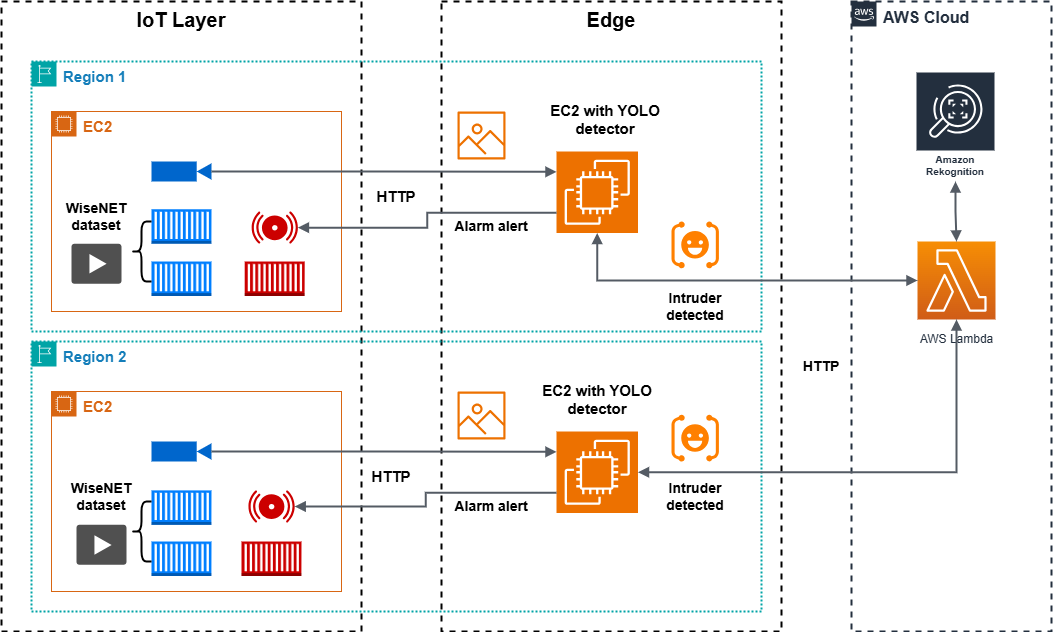
\includegraphics[width=0.75\textwidth]{./res/DS_architecture_version2.png}\\
\end{center}
\end{frame}

\begin{frame}
\frametitle{System architecture 2}
Final system architecture:


%TODO: add updated arch.
\begin{center}
    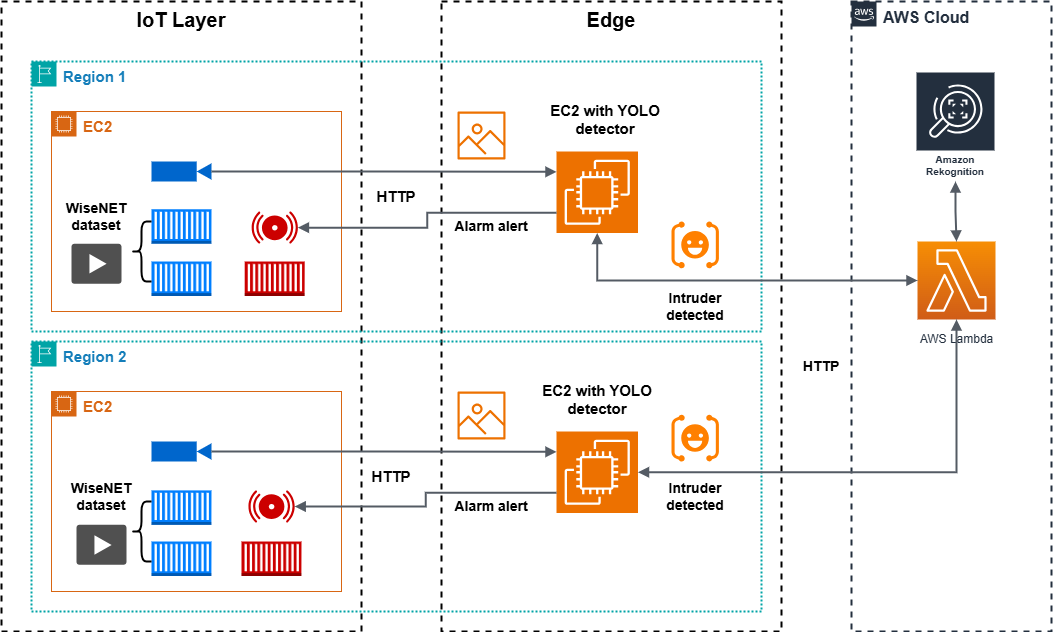
\includegraphics[width=0.75\textwidth]{./res/DS_architecture_version2.png}\\
\end{center}
\end{frame}



\section{Implementation details}

\begin{frame}
\frametitle{IOT - Edge}
\begin{itemize}
    \item socketIO for communication
    \item bla bla
\end{itemize}

\includegraphics[width=1\textwidth]{./res/socket-io-logo-1.jpeg}
\end{frame}


\begin{frame}
    \frametitle{Edge - IOT}
    \begin{itemize}
        \item Flask Rest Api
        \item bla bla
    \end{itemize}
    
\includegraphics[width=0.65\textwidth]{./res/flask.png}
\end{frame}

\begin{frame}
\frametitle{IoT Implementation Highlights}
\textbf{Frame Processing}
\begin{itemize}
    %\lstinputlisting[language=Python, firstline=86, lastline=93]{iot_code.py}
    \item Key Features:
    \begin{itemize}
    \item Configurable frame skip
    \item Real-time frame rate simulation
    \item Robust error handling
    \end{itemize}
    \end{itemize}

\textbf{Communication}
\begin{itemize}
    \item socket.io for communication between IOTs and Cloud.
    \item good for continuous dataflow
    \item setup once, then just send data
\end{itemize}
\begin{center}
    
\includegraphics[width=0.6\textwidth]{./res/socket-io-logo-1.jpeg}
\end{center}

\end{frame}

\begin{frame}
    \frametitle{Edge Server Architecture}
    \textbf{Async Processing Pipeline}
    \begin{itemize}

    \item two workers working asynchronously: 
    \begin{itemize}
        \item worker 1: Frame buffer queue
        \item worker 2: YOLO-based person detection
    \end{itemize}

    \item Cloud service integration
\end{itemize}

\textbf{Communication: Flask REST}
\begin{itemize}
    \item REST API for communication between EDGE and Cloud
    \item Edge sends HTTP request to Cloud $\rightarrow$ Cloud sends HTTP response
\end{itemize}
\begin{center}

    
\includegraphics[width=0.4\textwidth]{./res/flask.png}
\end{center}
% % TODO: incorporate this in the evaluation
%     \textbf{Performance Metrics}
%     \begin{itemize}
%     \item Detection ratios
%     \item Processing latency
%     \item Queue management
%     \end{itemize}

    \end{frame}

\begin{frame}
\frametitle{Cloud Service Features}

    \textbf{AWS Rekognition Integration}
    \begin{itemize}
    \item Face collection management 
    \item Known face indexing
    \item High-confidence matching
    \end{itemize}
    \textbf{Security Features}
    \begin{itemize}
    \item Configurable confidence thresholds
    \item Automatic collection management
    \item Error handling and logging
    \end{itemize}

\end{frame}


\begin{frame}
    \frametitle{Example Workflow/ Controlgraph}
    example of intruder detection. what happens at: 
    \begin{itemize}
        \item IOT? what are steps there
        \item EWDGE? what are the possible steps
        \item Cloud
        \item back to edge and alarm, why and how
    \end{itemize}
\end{frame}


\section{Performance Evaluation}
\begin{frame}
\frametitle{System Performance}
current blueprint generated by GenAI
    \begin{itemize}
    \item \textbf{Detection Metrics}
    \begin{itemize}
    \item YOLO detection ratio
    \item Face recognition accuracy
    \item Processing latency
    \end{itemize}
    \item \textbf{System Reliability}
    \begin{itemize}
    \item Connection resilience
    \item Error handling effectiveness
    \item Resource utilization
    \end{itemize}
    \item \textbf{Scalability}
    \begin{itemize}
    \item Multiple camera support
    \item Queue performance
    \item Cloud service responsiveness
    \end{itemize}
    \end{itemize}
\end{frame}

\section{Evaluation}

\begin{frame}
\frametitle{Evaluation}
\end{frame}


\bibliography{main}

\end{document}
